\documentclass[notes,11pt, aspectratio=169]{beamer}

\usepackage{pgfpages}
% These slides also contain speaker notes. You can print just the slides,
% just the notes, or both, depending on the setting below. Comment out the want
% you want.
\setbeameroption{hide notes} % Only slide
%\setbeameroption{show only notes} % Only notes
%\setbeameroption{show notes on second screen=right} % Both

\usepackage{helvet}
\usepackage[default]{lato}
\usepackage{array}
\usepackage{tgbonum}

\usepackage{tikz}
\usepackage{verbatim}
\setbeamertemplate{note page}{\pagecolor{yellow!5}\insertnote}
\usetikzlibrary{positioning}
\usetikzlibrary{snakes}
\usetikzlibrary{calc}
\usetikzlibrary{arrows}
\usetikzlibrary{decorations.markings}
\usetikzlibrary{shapes.misc}
\usetikzlibrary{matrix,shapes,arrows,fit,tikzmark}
\usepackage{amsmath}
\usepackage{mathpazo}
\usepackage{hyperref}
\usepackage{lipsum}
\usepackage{multimedia}
\usepackage{graphicx}
\usepackage{multirow}
\usepackage{graphicx}
\usepackage{dcolumn}
\usepackage{bbm}
\newcolumntype{d}[0]{D{.}{.}{5}}

\usepackage{changepage}
\usepackage{appendixnumberbeamer}
\newcommand{\beginbackup}{
   \newcounter{framenumbervorappendix}
   \setcounter{framenumbervorappendix}{\value{framenumber}}
   \setbeamertemplate{footline}
   {
     \leavevmode%
     \hline
     box{%
       \begin{beamercolorbox}[wd=\paperwidth,ht=2.25ex,dp=1ex,right]{footlinecolor}%
%         \insertframenumber  \hspace*{2ex} 
       \end{beamercolorbox}}%
     \vskip0pt%
   }
 }
\newcommand{\backupend}{
   \addtocounter{framenumbervorappendix}{-\value{framenumber}}
   \addtocounter{framenumber}{\value{framenumbervorappendix}} 
}


\usepackage{graphicx}
\usepackage[space]{grffile}
\usepackage{booktabs}
\newcommand\independent{\protect\mathpalette{\protect\independenT}{\perp}}
\def\independenT#1#2{\mathrel{\rlap{$#1#2$}\mkern2mu{#1#2}}}
\DeclareMathOperator{\Supp}{Supp}


\newtheorem{assN}{Assumption}
% These are my colors -- there are many like them, but these ones are mine.
\definecolor{blue}{RGB}{0,114,178}
\definecolor{red}{RGB}{213,94,0}
\definecolor{yellow}{RGB}{240,228,66}
\definecolor{green}{RGB}{0,158,115}

\hypersetup{
  colorlinks=false,
  linkbordercolor = {white},
  linkcolor = {blue}
}


%% I use a beige off white for my background
\definecolor{MyBackground}{RGB}{255,253,218}

%% Uncomment this if you want to change the background color to something else
%\setbeamercolor{background canvas}{bg=MyBackground}

%% Change the bg color to adjust your transition slide background color!
\newenvironment{transitionframe}{
  \setbeamercolor{background canvas}{bg=yellow}
  \begin{frame}}{
    \end{frame}
}

\setbeamercolor{frametitle}{fg=blue}
\setbeamercolor{title}{fg=black}
\setbeamertemplate{footline}[frame number]
\setbeamertemplate{navigation symbols}{} 
\setbeamertemplate{itemize items}{-}
\setbeamercolor{itemize item}{fg=blue}
\setbeamercolor{itemize subitem}{fg=blue}
\setbeamercolor{enumerate item}{fg=blue}
\setbeamercolor{enumerate subitem}{fg=blue}
\setbeamercolor{button}{bg=MyBackground,fg=blue,}



% If you like road maps, rather than having clutter at the top, have a roadmap show up at the end of each section 
% (and after your introduction)
% Uncomment this is if you want the roadmap!
% \AtBeginSection[]
% {
%    \begin{frame}
%        \frametitle{Roadmap of Talk}
%        \tableofcontents[currentsection]
%    \end{frame}
% }
\setbeamercolor{section in toc}{fg=blue}
\setbeamercolor{subsection in toc}{fg=red}
\setbeamersize{text margin left=1em,text margin right=1em} 

\newenvironment{wideitemize}{\itemize\addtolength{\itemsep}{10pt}}{\enditemize}

\usepackage{environ}
\NewEnviron{videoframe}[1]{
  \begin{frame}
    \vspace{-8pt}
    \begin{columns}[onlytextwidth, T] % align columns
      \begin{column}{.70\textwidth}
        \begin{minipage}[t][\textheight][t]
          {\dimexpr\textwidth}
          \vspace{8pt}
          \hspace{4pt} {\Large \sc \textcolor{blue}{#1}}
          \vspace{8pt}
          
          \BODY
        \end{minipage}
      \end{column}%
      \hfill%
      \begin{column}{.38\textwidth}
        \colorbox{green!20}{\begin{minipage}[t][1.2\textheight][t]
            {\dimexpr\textwidth}
            Face goes here
          \end{minipage}}
      \end{column}%
    \end{columns}
  \end{frame}
}

\title[]{\textcolor{blue}{Supervised Machine Learning II: \\ Heterogeneous Treatment Effects}} \author[PGP]{}
\institute[FRBNY]{\small{\begin{tabular}{c}
                           Paul Goldsmith-Pinkham  \\
\end{tabular}}}

\date{\today}

\begin{document}

%%% TIKZ STUFF
\tikzset{   
        every picture/.style={remember picture,baseline},
        every node/.style={anchor=base,align=center,outer sep=1.5pt},
        every path/.style={thick},
        }
\newcommand\marktopleft[1]{%
    \tikz[overlay,remember picture] 
        \node (marker-#1-a) at (-.3em,.3em) {};%
}
\newcommand\markbottomright[2]{%
    \tikz[overlay,remember picture] 
        \node (marker-#1-b) at (0em,0em) {};%
}
\tikzstyle{every picture}+=[remember picture] 
\tikzstyle{mybox} =[draw=black, very thick, rectangle, inner sep=10pt, inner ysep=20pt]
\tikzstyle{fancytitle} =[draw=black,fill=red, text=white]
%%%% END TIKZ STUFF

% Title Slide
\begin{frame}
\maketitle
\end{frame}

\begin{frame}{Machine Learning + Causality}
  \begin{wideitemize}
  \item Today, focusing on how to tie machine learning methods into estimation of causal effects
  \item Most of our ideas revolve around how to think about estimating CATEs -- conditional average treatment effects
    \begin{itemize}
    \item Why is this interesting? Why is knowing CATEs preferable to ATEs?
    \end{itemize}
  \item Recall that with exhaustively defined CATEs, we can estimate our ATE
    \begin{itemize}
    \item But, crucially, we could \emph{target} appropriately
    \item Well-estimated CATEs help identify better decisions based on decision rules
    \item Also good for economic theory!      
    \end{itemize}
  \item But, can be hard to do in a disciplined way
  \end{wideitemize}
\end{frame}

\begin{frame}{Why can ML be powerful in this space?}
  \begin{wideitemize}
  \item A serious concern in empirical work is specification hunting
    -- looking for significant effects in subgroups, and then telling
    a story about it
  \item One solution is pre-analysis plans -- tying our hands before
    the fact about what we will look at
  \item However, sometimes we would like to let the ``data speak''
    \begin{itemize}
    \item What if we could automate the process for estimating signficant CATEs?
    \end{itemize}
  \item Machine learning could allow us to estimate these approaches
    in a standardized way, while using out-of-sample testing to ensure
    that we are not data mining
  \end{wideitemize}
\end{frame}

\begin{frame}{The literatures with Machine learning and CATEs}
    \begin{columns}[onlytextwidth, T] % align columns
      \begin{column}{.9\textwidth}
        \begin{wideitemize}
        \item Today, will talk about two papers/lits:
          \begin{itemize}
          \item  Causal Trees (From Athey and Imbens (2016)
            \begin{itemize}
            \item More generally in the space of causal partitioning
            \item Causal ``Forests'' by Wager and Athey (2019) as well  
            \end{itemize}
          \item  GATES and CLAN from Chernozhukov et al. (2020)
            \begin{itemize}
            \item GATES = Sorted Group Average Treatment Effects
            \item CLAN = Classification Analysis
            \end{itemize}
          \end{itemize}
        \item These approaches are similarly focusing on CATEs, but
          solving a crucial statistical problem in two distinct ways
        \end{wideitemize}
      \end{column}%
      \hfill%
      \begin{column}{.5\textwidth}
      \end{column}%
    \end{columns}
\end{frame}

\begin{frame}{Machine learning and CATEs}
    \begin{columns}[onlytextwidth, T] % align columns
      \begin{column}{.9\textwidth}
        \begin{wideitemize}
        \item What is the statistical problem? There are two (related) issues:
          \begin{enumerate}
          \item Inference: even if we predict or show the effect of a
            treatment is higher in one subgroup than another, can we
            say whether this is just due to random variation, or a
            meaningful difference?
          \item Testing causal inference out-of-sample: Evaluating how
            ``accurate'' you are requires knowing your target
            outcome. E.g. $Y_{i} - \hat{Y}_{i}$. But,
            $\tau_{i} = Y_{i}(1) - Y_{i}(0)$ is fundamentally unknown. 
          \end{enumerate}
        \item These issues are in large part solved by additional
          sample splitting
        \item Importantly: these approaches do \emph{not} solve the
          issue of exogeneous variation
          \begin{itemize}
          \item In most settings, this should be viewed as a setting
            where we have a randomly varying treatment (e.g. an RCT)
            and we want to study CATEs
          \item However, if we have a good IV, we could study the
            reduced form quite sensibly!
          \end{itemize}
        \end{wideitemize}
      \end{column}%
      \hfill%
      \begin{column}{.5\textwidth}
      \end{column}%
    \end{columns}
\end{frame}

\begin{frame}{Causal trees (Athey and Imbens (2016)}
    \begin{columns}[onlytextwidth, T] % align columns
      \begin{column}{.5\textwidth}
        \begin{wideitemize}
        \item Necessary notation: Binary treatment, $D_{i}$, and covariates
          (potentially high dimensional) $X_{i}$. Outcome
          $Y_{i}$.
        \item In our discussion, we'll assume completely random assignment
          of $D_{i}$, but it is possible to account for conditioning
          variables as well using a p-score method 
        \item The key approach will be following the tree-based approach from last class, but with some essential modifications
          \begin{itemize}
          \item Recall that trees worked by splitting up observations at a
            given node based on a given characteristic
          \end{itemize}
        \end{wideitemize}
      \end{column}%
      \hfill%
      \begin{column}{.5\textwidth}
        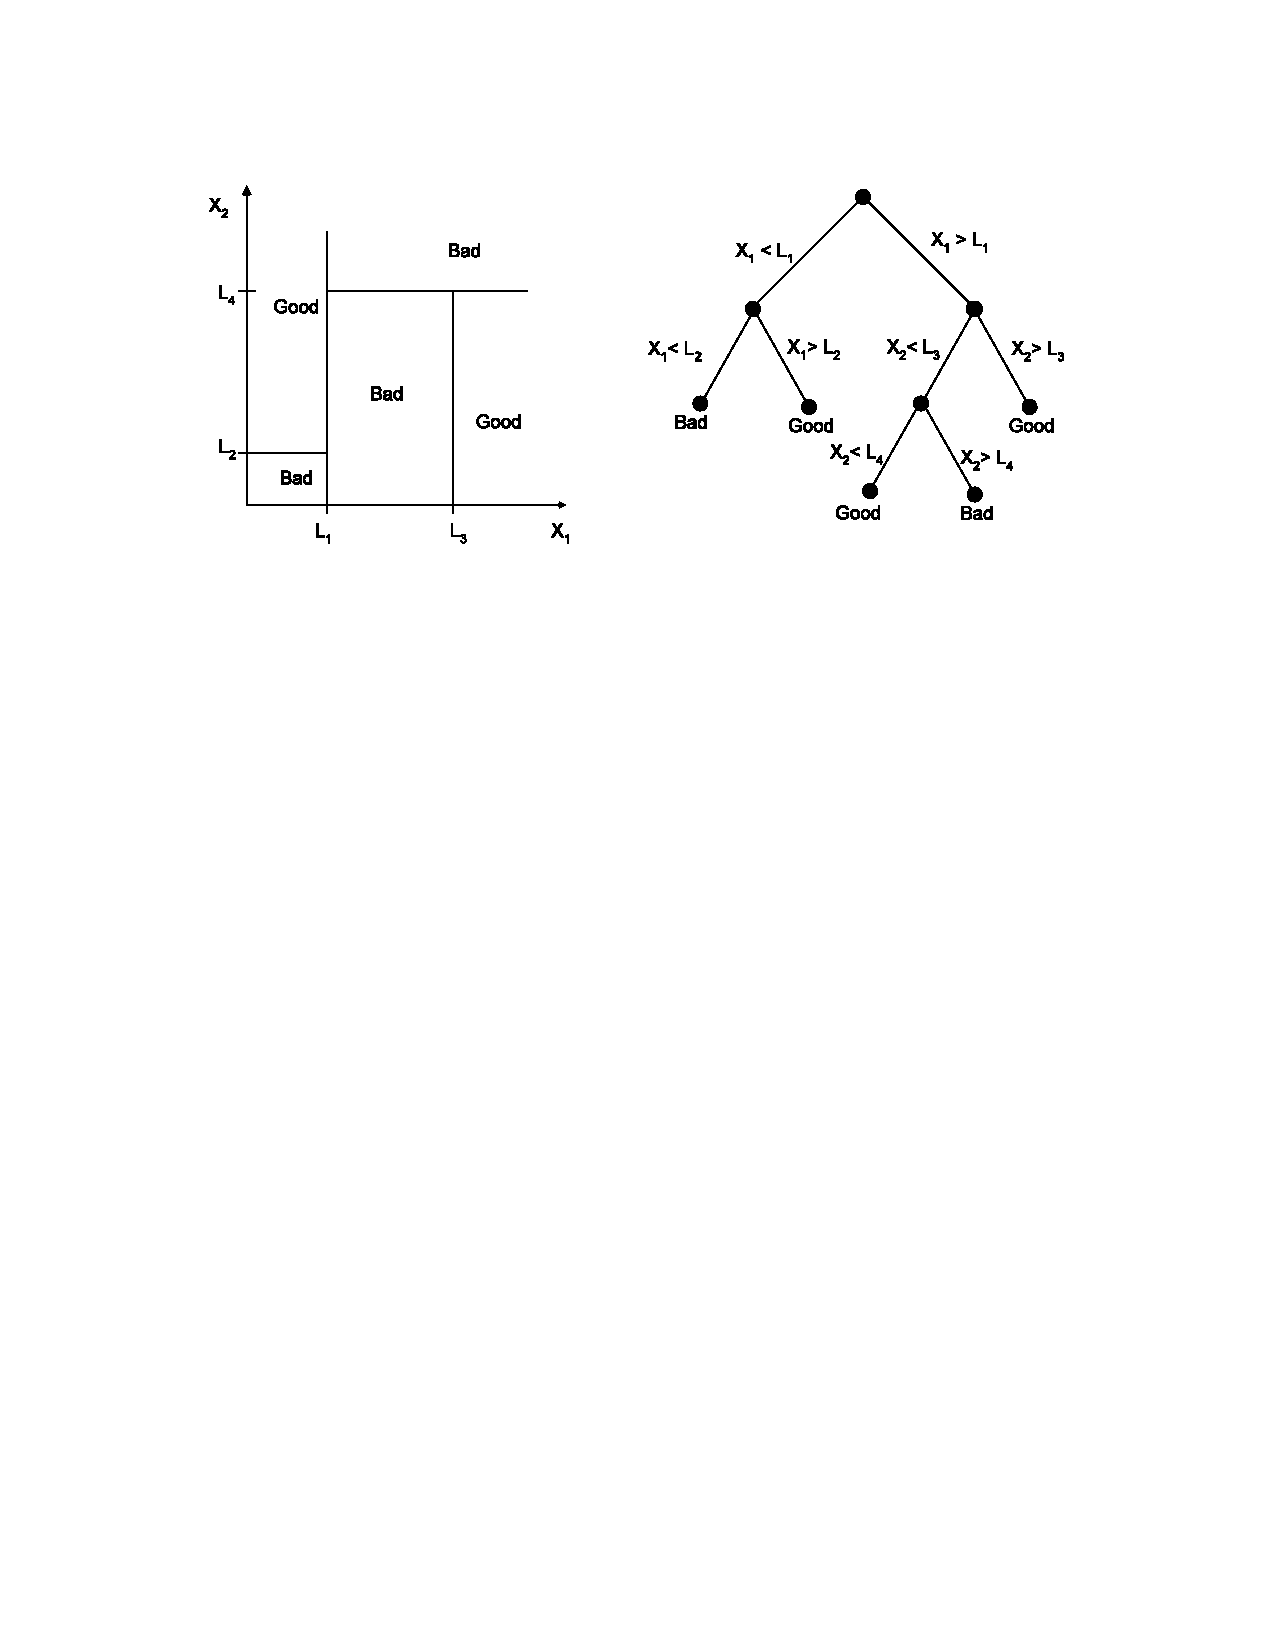
\includegraphics[width=\linewidth]{images/Tree_Lo.pdf}
      \end{column}%
    \end{columns}
\end{frame}


\begin{frame}{Causal trees (Athey and Imbens (2016)}
    \begin{columns}[onlytextwidth, T] % align columns
      \begin{column}{.8\textwidth}
        \begin{wideitemize}
        \item Key insight of this paper: when you choose what to split
          on, you are picking something that is ``unusual'' relative
          to the underlying data generating process
          \begin{itemize}
          \item This induces bias!
          \end{itemize}
        \item To see this, first focus on estimation of means, and 
          consider a simple example where $X$ is a simple dummy
          variable. You can either split on it, or not split on it.
          \begin{itemize}
          \item Imagine you split on it if $\bar{Y}_{1} - \bar{Y}_{0} > c$, some cutoff
          \end{itemize}
        \item On average, while each one is consistent, if you split
          only when the difference is large, you'll be selecting on a
          subset that will be biased relative to the population
        \item Key idea: split the sample into a training and test sample
          \begin{itemize}
          \item Use the training sample to decide on where to split
          \item Use the test to calculate means and evaluate the fit
          \end{itemize}
        \end{wideitemize}
      \end{column}%
      \hfill%
      \begin{column}{.5\textwidth}
      \end{column}%
    \end{columns}
\end{frame}

\begin{frame}{Causal trees (Athey and Imbens (2016)}
    \begin{columns}[onlytextwidth, T] % align columns
      \begin{column}{.7\textwidth}
        \begin{wideitemize}
        \item Algorithmically, the approach trades off between the following issues:
          \begin{itemize}
          \item Tree / Forest approaches overfit within sample
            \begin{itemize}
            \item Shows up in depth
            \item Shows up in means of splits
            \end{itemize}
          \item The algorithm focuses just on splitting within a leaf
            \begin{itemize}
            \item Ignores the fact that making many splits will create
              a lot of overall variance (that may not be meaningful)
            \end{itemize}
          \end{itemize}
        \item Sample splitting will address these issues
          \begin{itemize}
          \item Sample split to get consistent estimates
          \item Sample split to penalize too much depth and overall variance
          \end{itemize}
        \item Key payout: results will be pointwise consistent!
          \begin{itemize}
          \item In Wager and Athey's Causal Forests, will also have
            asymptotically normal distributions as well
          \end{itemize}
        \end{wideitemize}
      \end{column}%
      \hfill%
      \begin{column}{.5\textwidth}
      \end{column}%
    \end{columns}
\end{frame}


\begin{frame}{Causal trees (Athey and Imbens (2016)}
    \begin{columns}[onlytextwidth, T] % align columns
      \begin{column}{.5\textwidth}
        \begin{wideitemize}
        \item<1-> How to implement? In \texttt{R}, there's a very nice
          package that includes the Random Forest (see Wager and Athey (2019)) approach as well:
          \url{https://grf-labs.github.io/grf/}
        \item<2-> For \texttt{Python}, the \texttt{econml} package can do
          this as well (as well as many other approaches):
          \url{https://econml.azurewebsites.net/spec/spec.html}
        \item<3-> Nothing in Stata, sorry
        \end{wideitemize}
      \end{column}%
      \hfill%
      \begin{column}{.5\textwidth}
        \only<1>{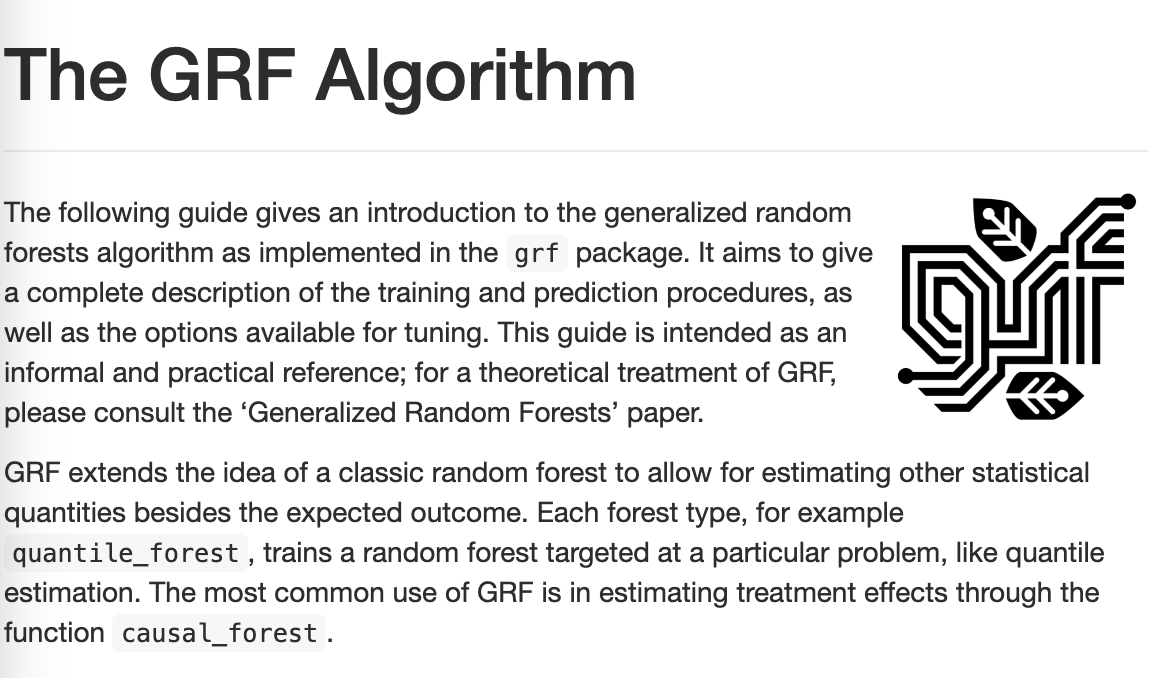
\includegraphics[width=\linewidth]{images/grf.png}}
        \only<2>{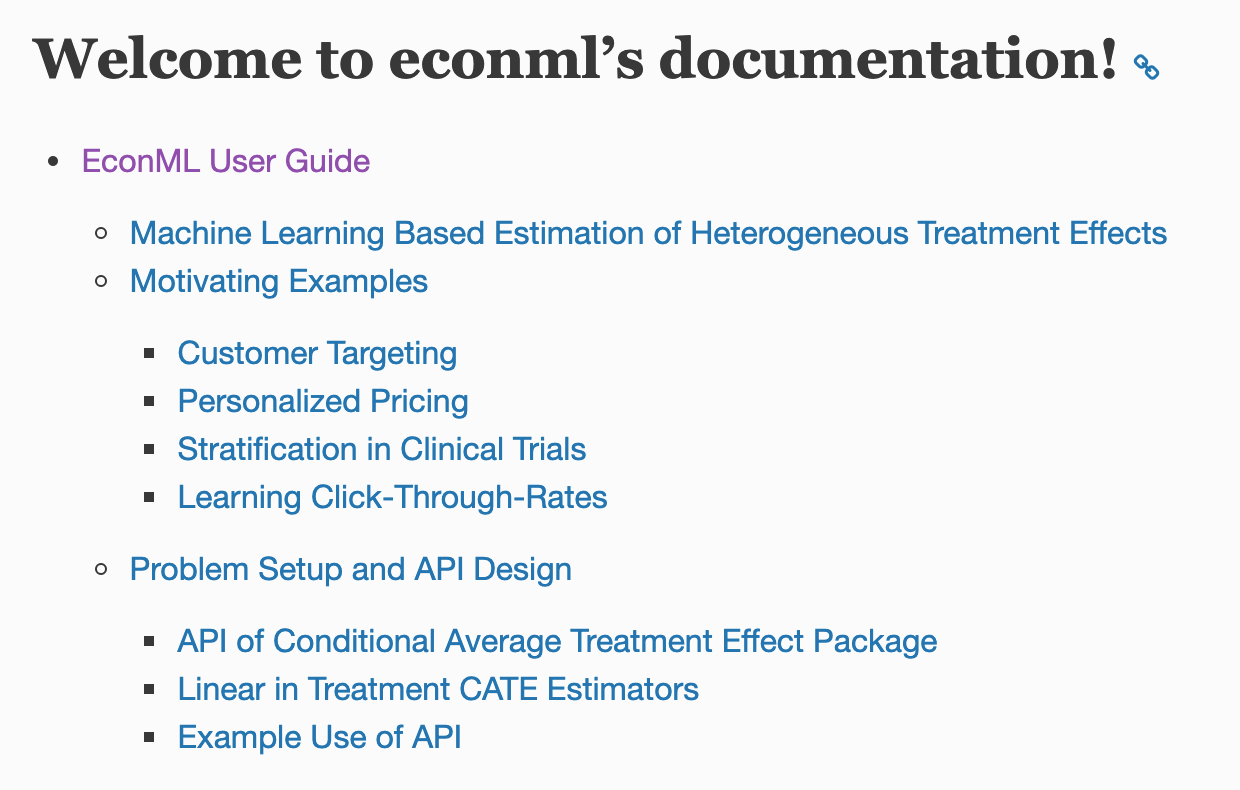
\includegraphics[width=\linewidth]{images/econml.png}}
        \only<3>{
\includegraphics[width=\linewidth]{images/frown.png}}
      \end{column}%
    \end{columns}
\end{frame}

\begin{frame}{GATES and CLAN (Chernozhukov et al. (2020)}
  \begin{wideitemize}
  \item The causal tree approach is a beautiful approach in solving
    the bias and infernece issues
  \item However, the general inference solution does not account for
    the uncertainty in the binning of the covariates
    \begin{itemize}
    \item Recall how the method works -- by using a split sample to
      choose the bins, the CATEs within those bins work just as well
      as any standard regression approach
    \item But this fails to account for the fact that these bins may
      change in different samples
    \item Consider how much your CATE changes if the cutoff point had
      changed slightly
    \end{itemize}
  \item Chernozhukov et al. (2020) highlight this issue, and propose a
    much more general approach
    \begin{itemize}
    \item This approach has more limitations, but at the benefit of
      being even more general
    \end{itemize}
  \end{wideitemize}
\end{frame}

\begin{frame}{GATES and CLAN  (Chernozhukov et al. (2020)}
  \begin{wideitemize}
  \item The key concept is that instead of trying to identify the
    CATEs directly, identify the key features of the CATEs instead
    \begin{itemize}
    \item More precisely, identify how much heterogeneity there is in
      the underlying estimates
    \item Then, figure out the characteristics of those groups with
      heterogeneous effects
    \end{itemize}
  \item The key approach starts with the following concept:
    \begin{itemize}
    \item Randomly split the sample into a main and auxiliary sample
    \item In the auxiliary sample, estimate the control mean, $B(X)$,
      and the treatment effect $S(X)$ (note that $S(X)$ will just be
      the treatment mean minus the control mean)
    \end{itemize}      
  \item This really just entails prediction of the control and
    treatment means for each group using an ML method
  \item Hence, we estimate $\hat{B}(X)$ and $\hat{S}(X)$ using a
    training sample, and then use the test sample to predict the
    actual values
  \end{wideitemize}
\end{frame}

\begin{frame}{BLP  (Chernozhukov et al. (2020)}
    \begin{columns}[onlytextwidth, T] % align columns
      \begin{column}{.5\textwidth}
  \begin{wideitemize}
  \item Crucially, the punchline is that $\hat{B}(X)$ and $\hat{S}(X)$
    will be biased, the inputs from the training sample are
    uncorrelated with the estimation error
  \item This implies that for a given observation in the training
    sample, $\hat{B}(X_{i})$ and $\hat{S}(X_{i})$ are useful summary
    statistics (projections) for that observation.
  \item What the paper shows is that if you take these measures and
    run the following regression, you can identify whether there is
    meaningful heterogeneity
  \end{wideitemize}
      \end{column}%
      \hfill%
      \begin{column}{.5\textwidth}
        \only<1>{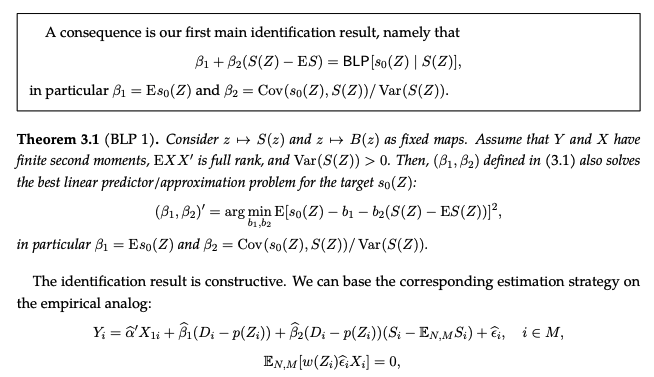
\includegraphics[width=\linewidth]{images/chernozhukov_Blp.png}}
        \only<2>{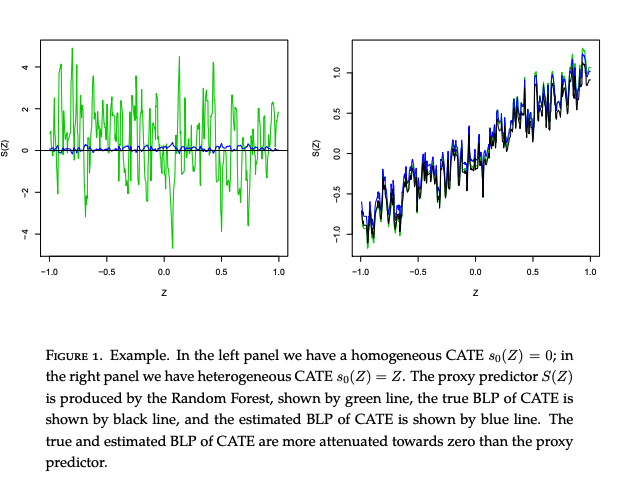
\includegraphics[width=\linewidth]{images/chernozhukov_Blp2.png}}
      \end{column}%
    \end{columns}
\end{frame}


\begin{frame}{GATES and CLAN}
    \begin{columns}[onlytextwidth, T] % align columns
      \begin{column}{.5\textwidth}
  \begin{wideitemize}
  \item If we identify heterogeneity, we'd like to know which $X$
    drive it.  The problem is that $\tau(X)$ is very high-dimensional
  \item The GATES approach says -- what if we grouped the effects into
    bins $G$, increasing in effect size.
    \begin{itemize}
    \item We can talk about the property of these GROUPED average treamtent effects, which average of the high dimensional properties
    \item In turns out we can say a lot about that, statistically
    \end{itemize}
  \item Moreover, we can test for whether these are all the same
    \begin{itemize}
    \item Harkens back to binscatter and testing for monotonicity!
    \end{itemize}
  \end{wideitemize}
      \end{column}%
      \hfill%
      \begin{column}{.5\textwidth}
        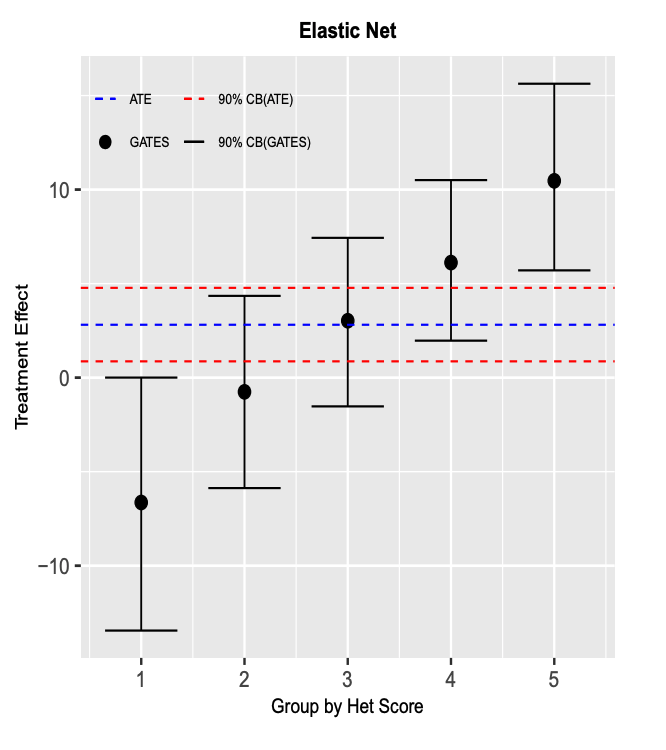
\includegraphics[width=\linewidth]{images/GATES.png}
      \end{column}%
    \end{columns}
\end{frame}

\begin{frame}{GATES and CLAN}
    \begin{columns}[onlytextwidth, T] % align columns
      \begin{column}{.5\textwidth}
  \begin{wideitemize}
  \item The issue is that we still haven't solved for what these groups are
    \begin{itemize}
    \item Knowledge of heterogeneity doesn't get us very far
    \end{itemize}
  \item The CLAN approach asks how important characteristics vary by
    these binned groups
  \item We can use this to identify bins worth targetting
  \end{wideitemize}
      \end{column}%
      \hfill%
      \begin{column}{.5\textwidth}
        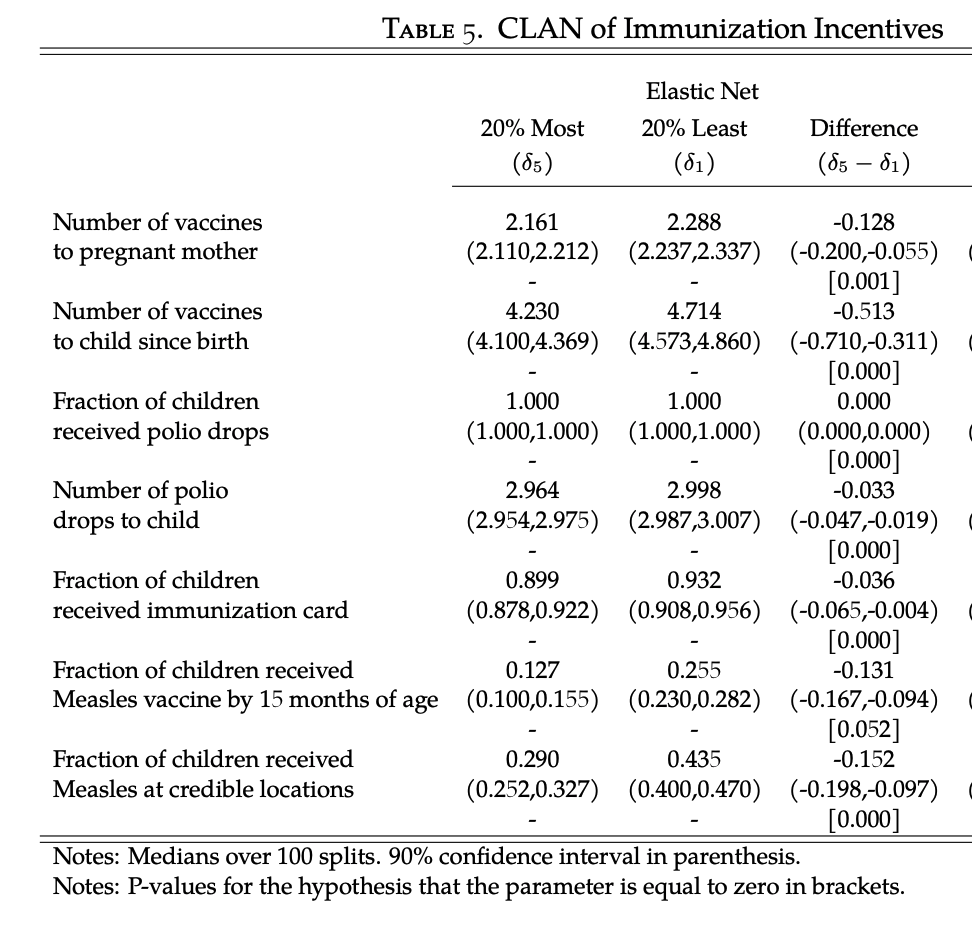
\includegraphics[width=\linewidth]{images/CLAN.png}
      \end{column}%
    \end{columns}
\end{frame}

\begin{frame}{Implementation in practice}
  \begin{wideitemize}
  \item Chernozhukov et al. (2020) outline the algorithm in detail in the paper
  \item Code is available here from Mert Demirer
    (\url{https://github.com/demirermert/MLInference/blob/master/Heterogeneity/EL1.R})
  \item Important note -- still need conditional exogeneity / strict ignorability!
  \end{wideitemize}
  
\end{frame}


\end{document}